\section{ローパスフィルタのによる画像処理}

\autoref{code:low_pass}に,画像に対してローパスフィルタを行う$\mathsf{low\_pass\_img}()$関数を示す.
\autoref{code:low_pass}では,\autoref{code:low_pass}と同様に
入力された画像の周波数成分を抽出し, $x, y$それぞれのカットオフ周波数より高い周波数領域
に0を代入したのちに逆変換を用いて画像へと復元する.
\lstinputlisting[caption=画像へのローパスフィルタを行う$\mathsf{low\_pass\_img}()$関数, label={code:low_pass}]{script/show_low_pass.py}

\autoref{fig:low_input}に入力画像,
\autoref{fig:low_pass_dft}に\autoref{fig:dft_low}に対してローパスフィルタで
処理した後の周波数成分,
\autoref{fig:low_pass_idft}に復元した出力画像を示す.
\autoref{fig:low_pass_idft}と\autoref{fig:low_input}を比較すると,
画像内の輪郭がぼやけており鮮明さが失われていることがわかる.
このことから,画像データに対してローパスフィルタを用いると画像に対してぼかしをかける
処理として活用することができる.

\iffigure
\begin{figure}[h]
  \centering
  \begin{minipage}{.25\hsize}
    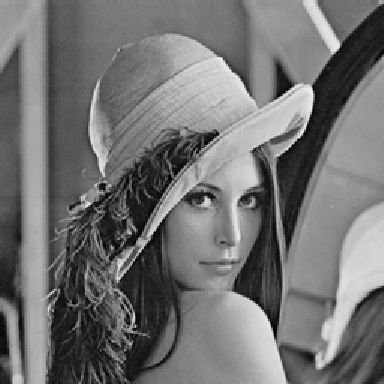
\includegraphics[clip, width=\textwidth]{figure/Lenna.pdf}
    \caption{入力画像}
    \label{fig:low_input}
  \end{minipage}
  \begin{minipage}{.25\hsize}
    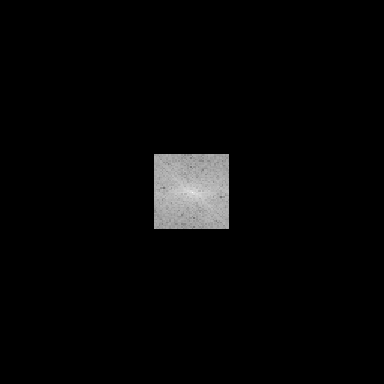
\includegraphics[clip, width=\textwidth]{figure/low_pass_dft_2d.pdf}
    \caption{ローパスフィルタによる抽出}
    \label{fig:low_pass_dft}
  \end{minipage}
  \begin{minipage}{.25\hsize}
    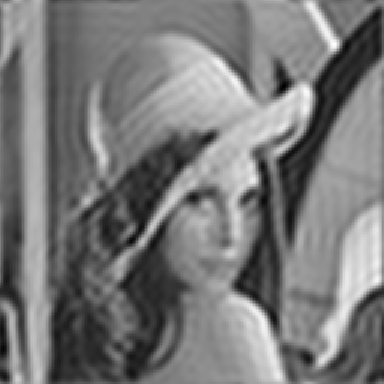
\includegraphics[clip, width=\textwidth]{figure/low_pass_idft_2d.pdf}
    \caption{処理後の画像}
    \label{fig:low_pass_idft}
  \end{minipage}
\end{figure}
\fi
